
Due to the very short time we had to complete this project, we couldn't collect as much training data as we wanted. Partly also because of problems with the Raspberry Pi's timezone setting over Ethernet. Our final tree reflects just that constrained enviroment. Despite only turning the lights on at 2 distinct junctions, the tree still achieves a 91\% accuracy on the trained data.

\begin{figure}
  \centering
    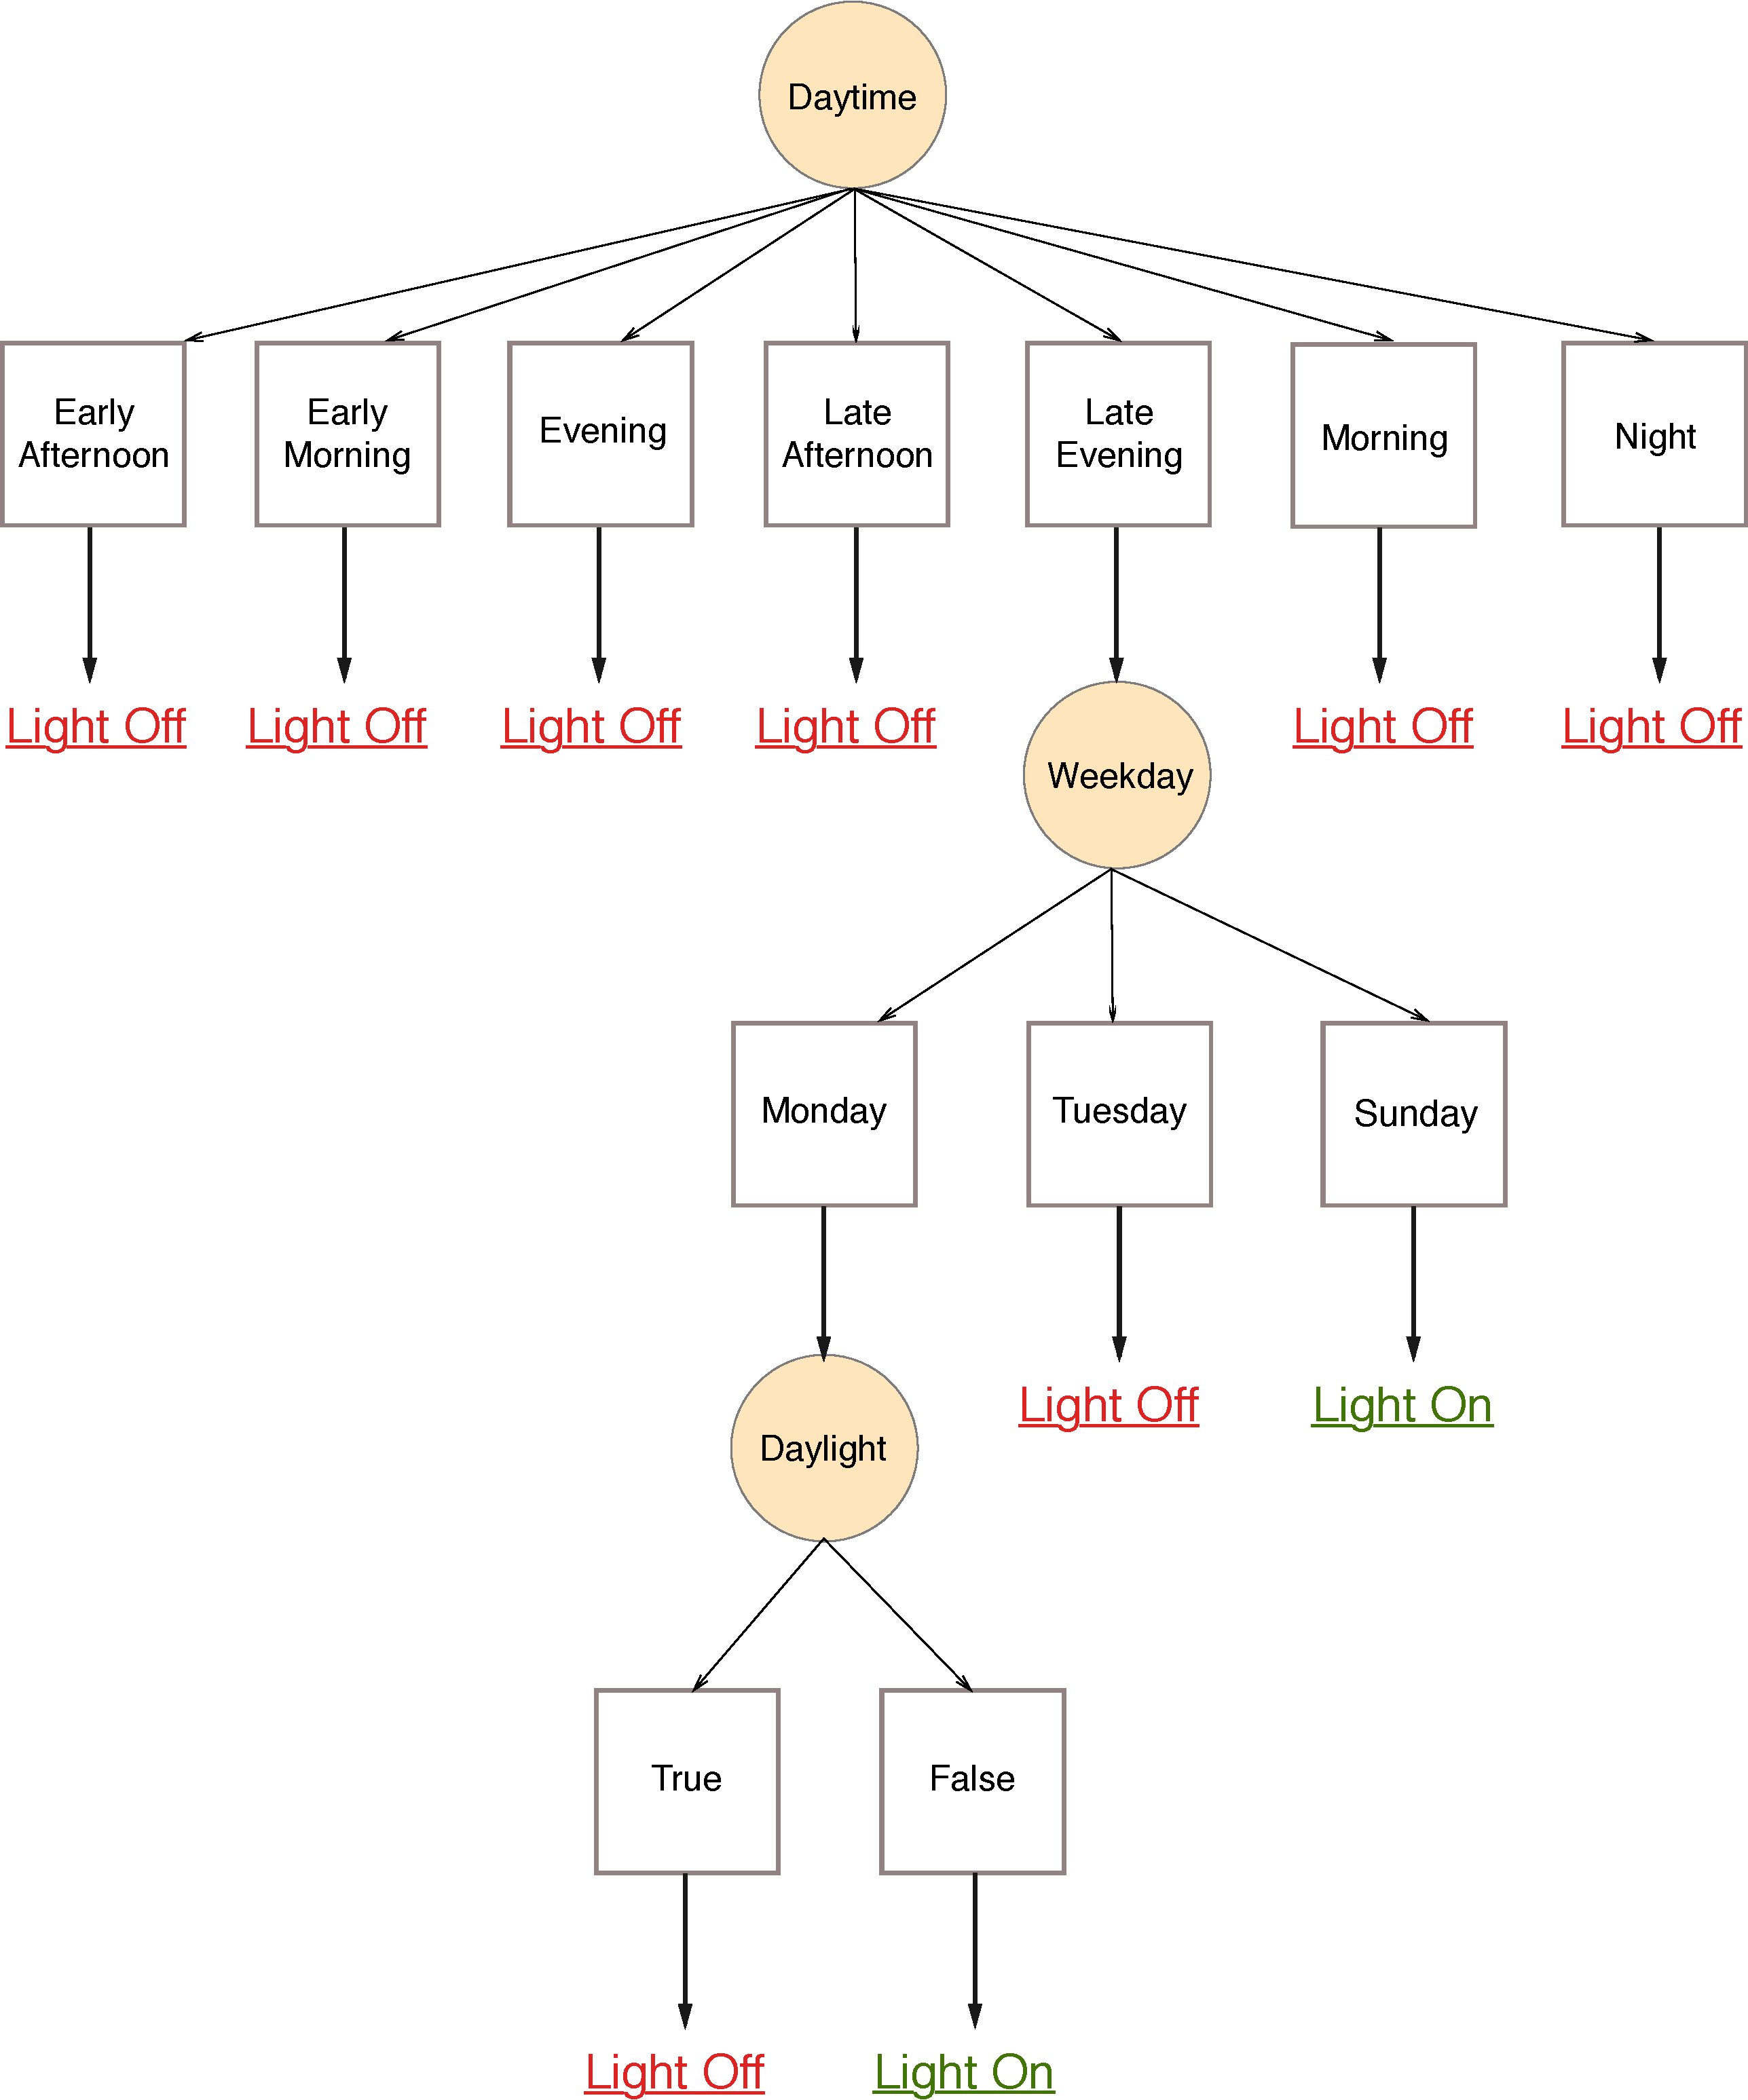
\includegraphics[width=1.0\textwidth]{img/tree.pdf}
  \caption{Resulting decision tree}
  \label{fig:result}
\end{figure}

Interesting would be a result with complete full week long training.

\subsection{Future Work}

Future work could improve the SMART Machine Learning Lamp in the following ways.

The lamps underlying decision tree model currently cannot be easily adjusted after the initial training, without a complete new training-phase. Future work could improve upon that, and continuously improve the model with the help of ongoing user interaction with the lamp. This also includes when new devices that should impact the decision are brought to the household.




